\documentclass[12pt]{article}
%\usepackage[pdftex]{graphicx}
\usepackage{%
	amsfonts,%
	amsmath,%	
	amssymb,%
	amsthm,%
%	babel,%
	bbm,%
	%biblatex,%
	caption,%
	centernot,%
	color,%
	enumerate,%
	epsfig,%
	epstopdf,%
	etex,%
	geometry,%
	graphicx,%
	hyperref,%
	latexsym,%
	mathtools,%
	multicol,%
	pgf,%
	pgfplots,%
	pgfplotstable,%
	pgfpages,%
	proof,%
	psfrag,%
	subfigure,%	
	tikz,%
	ulem,%
	url%
}	

\usepackage[mathscr]{eucal}
\usepgflibrary{shapes}
\usetikzlibrary{%
  arrows,%
  backgrounds,%
  chains,%
  decorations.pathmorphing,% /pgf/decoration/random steps | erste Graphik
  decorations.text,%
  matrix,%
  positioning,% wg. " of "
  fit,%
  patterns,%
  petri,%
  plotmarks,%
  scopes,%
  shadows,%
  shapes.misc,% wg. rounded rectangle
  shapes.arrows,%
  shapes.callouts,%
  shapes%
}

\theoremstyle{plain}
\newtheorem{thm}{Theorem}[section]
\newtheorem{lem}[thm]{Lemma}
\newtheorem{prop}[thm]{Proposition}
\newtheorem{cor}[thm]{Corollary}

\theoremstyle{definition}
\newtheorem{defn}[thm]{Definition}
\newtheorem{conj}[thm]{Conjecture}
\newtheorem{exmp}[thm]{Example}
\newtheorem{assum}[thm]{Assumptions}
\newtheorem{axiom}[thm]{Axiom}

\theoremstyle{remark}
\newtheorem{rem}[thm]{Remark}
\newtheorem{note}[thm]{Note}

\newcommand{\norm}[1]{\left\lVert#1\right\rVert}
\newcommand{\indep}{\!\perp\!\!\!\perp}
\DeclarePairedDelimiter\abs{\lvert}{\rvert}%
%\DeclarePairedDelimiter\norm{\lVert}{\rVert}%
\newcommand{\tr}{\operatorname{tr}}
\newcommand{\R}{\mathbb{R}}
\newcommand{\Q}{\mathbb{Q}}
\newcommand{\N}{\mathbb{N}}
\newcommand{\E}{\mathbb{E}}
\newcommand{\Z}{\mathbb{Z}}
\newcommand{\B}{\mathscr{B}}
\newcommand{\C}{\mathcal{C}}
\newcommand{\T}{\mathscr{T}}
\newcommand{\F}{\mathcal{F}}
\newcommand{\G}{\mathcal{G}}
%\newcommand{\ba}{\begin{align*}}
%\newcommand{\ea}{\end{align*}}

% Debug
\newcommand{\todo}[1]{\begin{color}{blue}{{\bf~[TODO:~#1]}}\end{color}}


\makeatletter
\def\th@plain{%
  \thm@notefont{}% same as heading font
  \itshape % body font
}
\def\th@definition{%
  \thm@notefont{}% same as heading font
  \normalfont % body font
}
\makeatother
\date{}
\usepackage{tabu}
%\usepackage[demo]{graphicx}
\usepackage{caption}
%\usepackage{subcaption}
\usepackage{float}
\usepackage{amsmath}
\newcommand*\textfrac[2]{
  \frac{\text{#1}}{\text{#2}}
}

\begin{Huge}
	\title{SPQT PROJECT REPORT \\CHARACTERIZATION OF ECONOMY}
\end{Huge}

\begin{document}
\maketitle


\begin{large}
\begin{center}
	Manju M Raj\\
	Nanditha Unnikrishnan\\
\end{center}	
\end{large}



\newpage
\tableofcontents

\newpage

\section{INTRODUCTION}

On November 8$^{th}$,Indian government took a historic decision by announcing that the high-denomination notes (Rs. 500 and Rs. 1,000) then in circulation would cease to be legal tender.
With demonetization effort 86 percentage of Indian currency was nullified that aimed to wash the stock of ‘black market's cash supply’ and counterfeit notes out of the economy and convert it into the licit, banked and taxable, part of the economy.
The move has led to a shortage of lower denomination notes such as Rs 100 and Rs 50 that are still legal tender, as people have taken to conserving whatever cash they have in hand. The demonetization initiative has caused a sudden breakdown in India’s commerce and the unbanked and informal economy was hard hit. Trade across all aspects of the economy has interrupted, and sectors like agriculture, fishing, and the huge informal market were almost shut down during the initial days of announcement. The informal sector in India employs more than a majority of the workers and most transactions are in cash.
\\
Since our economy is heavily dependent on cash, as only less than half the population uses banking system for monetary transactions, demonetization hit trade and consumption hard. With people scrambling for cash to pay for goods and services, the move took a big toll on the country's growth and output during the then fiscal. 


\section{PROBLEM STATEMENT}
Our aim is to characterize the effects of demonetization on consumption. We want to predict out how much time it takes for the economy to stabilize after the disturbance caused by demonetization. \\
Majority of Indian population depends on cash-in-hand rather than banking system for consumption.
Therefore it is sufficient to model cash-in-hand as a stochastic process to study the effects.


\section{LITERATURE SURVEY}
\begin{itemize}
  \item \textit{Stochastic Implications of the Life Cycle-Permanent Income Hypothesis: Theory and Evidence (Robert E Hall)}\\
  The paper is based on the life cycle – permanent income hypothesis and models consumption as a random walk process. The paper suggests that no other information apart from the consumption at time 't' helps to predict the future consumption. The income or wealth in periods 't' or earlier are irrelevant.
  \paragraph{}
  For policy analysis, the pure life cycle permanent hypothesis supports the view that unexpected changes in policy, affect consumption only to the extent that they affect permanent income. But in the case of demonetization, the permanent income is not affected and hence, modeling consumption as random walk in the scenario with demonetization would provide false results.\\With the literature survey conducted by us, we were not able to find any paper which takes into     consideration the cash-in-hand (the only quantity directly affected by demonetization). Therefore we developed a new model of cash-in-hand as a Discrete Time Markov Process.
  \item To implement the model, data were collected from the website of Reserve Bank of India. Monetary policies regarding the limit on withdrawals from ATM during the months November 2016 –February 2017 were observed.
  \begin{table}[h]
\centering
\caption{Changes in Monetary Policy}
\begin{tabu} to 0.8\textwidth { | X[l] | X[c] | X[c] | X[c] | }
 \hline
  Date & Daily limit (in Rs.) & Limit of withdrawal from bank & Weekly limit (in Rs.) \\
 \hline
 10$^{th}$ Nov'16 & 2000 & 10000 & 20000 \\
 \hline
 18$^{th}$ Nov'16& 2500 & 10000 & 24000 \\
\hline 
  1$^{st}$ Jan'17& 4500  & 10000 & 24000 \\
\hline
 
 17$^{th}$ Jan'17 & 10000  & 10000 & 24000 \\
 \hline
 20$^{th}$ Feb'17& 10000  & 10000 & 50000 \\
 \hline
 13$^{th}$ Mar'17& 10000  & 10000 & No limit \\
 \hline
\end{tabu}
\end{table}

\item Mixing Time: \\
The mixing time of a Markov chain is defined as the time taken for the Markov chain to attain its stationary distribution.
\\\\Let $\lbrace$X$_{k}$,k$\geq$0$\rbrace$ be an irreducible, finite space DTMC with state space consiting of integers $\lbrace 1,2,3,\cdots,M\rbrace$.p$_{i,j}$ denotes the transition probability from state i to j and $\pi^{T}$ = [ $\pi_{1}$ $\pi_{2}$ $\cdots$ $\pi_{M}$ ] denotes the stationary distribution of the markov chain.In [1], the time to mixing is defined as follows:
\\\\Let Y be a random variable with probability mass function given by $\pi$. A  markov chain $\lbrace X_{k},k\geq0 \rbrace$ is said to achieve mixing, at time T = n, when $X_{n}$ = Y for the smallest such n $\geq$ 1.To find the mean mixing time starting from an initial state, sample a value from $\lbrace\pi_{j}\rbrace$ to get a value for Y, say Y = j. Observe the markov chain starting from any state, say i.\\ $T_{ij}$ is defined as the first time the markov chain reaches state j given the initial state i.  
\begin{center}
$T_{ij}$ = min$\lbrace$ n $\geq$ 1 such that $X_{n}$ = j given that $X_{0}$ = i$\rbrace$  
\end{center}
As  ${X_{k}, k\geq0}$  is an irreducible, finite space DTMC, $T_{ij}$ is an almost-surely finite random variable. $m_{ij}$ is defined as the expected value of $T_{ij}$.
\begin{center}
$m_{ij}$ = E [  $T_{ij}$ $|$ $X_{0}$ = i ]\\
\end{center}
$m_{ij}$ is the mean time it takes for the DTMC to reach state j from initial state i, i.e. the mean time to mix when the final state is j and initial state is i. Defining the statistic $\eta_{i}$ :
\begin{equation}
\eta_{i} = \sum_{j\in\textit{E}} m_{ij}\pi_{j}
\end{equation}
where $\eta_{i}$ is defined as mean mixing-time when the initial state is i. \\
Let \textbf{$\eta$} be the vector: $[$$\eta_{1}$ $\eta_{2}$ $\cdots$ $\eta_{M}$$]^{T}$.\\
\paragraph{}
In [1], a method has been described to calculate expected mixing time from the Transition Probability Matrix,P.\\ Define the following matrices and vectors:
\begin{itemize}
\item Vector $e^{T}$ =  [ 1 1 1 $\cdots$ 1]$_{(1 \times M)}$
\item E is the MxM all one matrix. E = e$e^{T}$ 
\item M is the matrix with element (i,j) as $m_{ij}$, which is the mean time taken to mix when the final state is j and initial state is i. \\
M = [$m_{ij}$]
\item Diagonal matrix M$_{d}$ has diagonal elements given by $m_{ii}$, i=1,2,3$\cdots$M.(mean time to mix given the initial and final state is i)\\
M$_{d}$=[$\delta_{ij}$m$_{ij}$]
\item $\Pi$ = e$\pi^{T}$
\end{itemize}
Next step is to calculate generalized inverse of (I-P).Let G be the g-inverse of (I-P).\\
(\textit{Generalized inverse (g-inverse) of a matrix A is D if ADA = A.} )\\
Compute the elements of another matrix ,H defined as 
\begin{center}
H = G( I - $\Pi$)
\end{center}
Compute the following matrices:
\begin{itemize}
\item C = I - H 
\item C$_{d}$=[$\delta_{ij}$C$_{ij}$]
\end{itemize}
Using the above matrices, matrix M can be computed as:
\begin{equation}
M = [ C - EC_{d} + E ].M_{d}
\end{equation}
$\eta_{i}$ ,which is the mean time to mix starting from state i, can be computed using the below equation:
\begin{equation}
\eta_{i} = M_{i}.\pi^{T} 
\end{equation}
where $M_{i}$ is the $i^{th}$ row of matrix M.
In [2],it has been proved that $\eta_{i}$s are independent of i.Therefore the expected mean time to mix starting from any state is the same: $\eta_{1}$ = $\eta_{2}$ = $\cdots$ = $\eta_{M}$ .\\
An alternate way to calculate mixing times has also been presented in [1].
For an irreducible Markov chain $\lbrace$X$_{n},n\geq0 \rbrace$,with p$_{j}$(n) = P$\lbrace$X$_{n}$ = j$\rbrace$, i.e . probability that the DTMC  takes the value j on the $n^{th}$ day, and stationary distribution $\lbrace\pi_{j}\rbrace$,entropy is defined as:
\begin{center}
E(n)= -$\Sigma_{j}$ p$_{j}$(n)log $\frac{p_{j}(n)}{\pi_{j}}$
\end{center}
For m $\geq$ 1, E(n + m) $\geq$ E(n), with equality if and only if p$_{j}$(n) = $\pi_{j}$ for all
j. Hence the “mixing time” is just the minimal integer such that the equality holds.In other words,if t is the mixing time,
\begin{center}
p$_{j}(t+x)$ = p$_{j}(t)$ = $\pi_{j}$, for any integer x$\geq$0.
\end{center}
In our case the step size of the DTMC is a single day and hence mixing time is defined in terms of number of days to achieve stationary distribution.The very next day after mixing has taken place, the total variation distance between the current distribution and the stationary distribution becomes very small. We have used this concept during the MATLAB simulations.
\end{itemize}

\section{SYSTEM MODEL}
The cash-in-hand is modeled as a Discrete Time Markov Process. The state space of this DTMC consists of the discretized versions of cash-in-hand as multiples of 500s truncated at Rs.10,000.
\begin{center}
\textit{E} = $\lbrace$ 500 $*$ n, n=0,1,2,3,$\cdots$ 20$\rbrace$
\end{center}
The Transition Probability Matrix of this DTMC is a 21x21 matrix.The transitions among these state spaces are caused by inflow of cash (mostly by ATM withdrawals) and consumption.\\
\paragraph{\textit{Arrival Process:}}
Withdrawal from banks and ATMs constitute the arrival process of this DTMC.The instants at which withdrawal takes place has been modelled as a Bernoulli process : ber(pwithdrawal) with parameter pwithdrawal defined as the probability of withdrawal of a non-zero amount.The amount withdrawn at each of these instants follows a probability mass function, calculated empirically, the details of which is given in section [5].
\paragraph{\textit{Departure Process:}}
The departure process of the DTMC is constituted by consumption.This has also been modelled as a Bernoulli process: ber(pconsumption) with parameter pconsumption defined as the probability of spending a non-zero amount.The amount spent each time follows a particular probability mass function( described in section[5]).
\paragraph{}
We have considered two separate scenarios: before and after demonetization (Nov 8th). 
Assume that the DTMC already follows stationary distribution before demonetization. 
On November 8$^{th}$, demonetization acted as a disturbance to the cash-in-hand DTMC which had achieved stationarity\textit{.The effect of demonetization as the disturbance has been modeled through changes in the Transition Probability Matrix.} \\We made observations in the time period of four months from November 2016 to February 2017, during which the economic policies deciding the limit of withdrawal from banks kept changing. With any change in the policy, the TPM also changes. By the end of February 2017, the withdrawal limits were restored to the values before demonetization.  We have assumed that after February 20$^{th}$ the TPM became almost same as the one before demonetization was put in effect, the DTMC may not have achieved stationary distribution though.\\ With a similar TPM and a different initial distribution, the mixing times can be calculated. The expected value of mixing time will provide an estimate of the time for the economy to stabilize.

\section{WORK DONE}
In this project we are considering only the middle class population. We collected bank statements of 100 people from October 2016 to February 2017. The tabulated data is given below:
(\textit{The values in each cell indicate the total number of times a particular amount has been withdrawn by 100 people in a given month. For example, in the month of Nov-Dec, the amount Rs.1500 was withdrawn a total of 16 times by 100 people.}) \\
Cash-in-hand has been modeled as a DTMC.
Let $\lbrace$P$_{k}$,k$\geq$0$\rbrace$ denote the DTMC under consideration. \textit{P$_{k}$} is the cash-in-hand on the \textit{k$^{th}$} day.\\
\begin{small}
\begin{table}[]
\centering
\caption{Withdrawal Data}

\begin{tabu} to 1\textwidth { | X[c] | X[c]  | X[c] | X[c] | X[c] | }
 \hline
 
 Withdrawal  & Oct-Nov & Nov-Dec & Dec-Jan & Jan-Feb \\
 \hline
 0 & 2524 & 2707 & 2706 & 2612 \\
 \hline
 500 & 110 & 80 & 106 & 106 \\
 \hline
 1000 & 80 & 27 & 49 & 68 \\
 \hline
 1500 & 55 & 16 & 35 & 42 \\
 \hline
 2000 & 67 & 93 & 102 & 127 \\
 \hline
 2500 & 15 & 37 & 14 & 42 \\
 \hline
 3000 & 28 & 5 & 8 & 13\\
 \hline
 3500 & 4 & 1 & 12 & 18 \\
 \hline
 4000 & 17 & 5 & 25 & 14 \\
 \hline
 4500 & 20 & 8 & 10 & 22 \\
 \hline
 5000 & 40 & 6 & 15 & 7 \\
 \hline
 5500 & 22 & 1 & 1 & 1 \\
 \hline
 6000 & 17 & 1 & 2 & 8 \\
 \hline
 6500 & 14 & 1 & 1 & 2 \\
 \hline
 7000 & 25 & 2 & 1 & 1 \\
 \hline
 7500 & 19 & 4 & 1 & 1 \\
 \hline
 8000 & 11 & 1 & 2 & 4 \\
 \hline
8500 & 9 & 1 & 1 & 1\\
 \hline
9000 & 2 & 1 & 1 & 2 \\
 \hline
 9500 & 1 & 1 & 1 & 1\\
 \hline
 10000 & 20 & 2 & 7 & 8 \\
 
 \hline
\end{tabu}
\end{table}
\paragraph{}
\textit{\textbf{Arrival Process:}} $\lbrace$A$_{k}$,k$\geq$0$\rbrace$ \\
    
    The arrival process is constituted by withdrawal from banks and ATMs.We are assuming that in-flow of cash can occur only due to withdrawals. \textit{A$_{k}$} is the cash withdrawn on \textit{k$^{th}$} day. The arrival process is modeled as a bernoulli process :ber(pwihtdrawal) with parameter \textit{pwihtdrawal} defined as
    \begin{center}
    pwithdrawal = 1 -  $\textfrac{No of days zero cash was withdrawn}{Total no of withdrawals }$
    \end{center}
   \textit{ For example, pwihdrawal in the month Nov-Dec is given by pwithdrawal = 1 - 2707/3100 = 0.1268 .}\\Total number of withdrawals is a constant equal to 3100 as we are assuming that if a particular day no cash is withdrawn, then it is counted as withdrawing zero cash.\\\\
    The amount withdrawn on each day is assumed to be an i.i.d process following a probability mass function which has been computed empirically.  
    \begin{center}
    P(A$_{k}$ = j ) = $\textfrac{No of times Rs. j was withdrawn in a particular month}{Total no of withdrawals}$
    \end{center}
    \textit{For example, in the month of Oct-Nov, P(A$_{k}$ = 3000) = 28 /3100 =0.009032}
 \begin{table}[H]
\centering
\caption{Consumption Data}

\begin{tabu} to 1\textwidth { | X[c] | X[c]  | X[c] | X[c] | X[c] | }
 \hline
 
Expenditure  & Oct-Nov & Nov-Dc & Dec-Jan & Jan-Feb \\
 \hline
 0 & 415 & 1141 & 1097 & 621 \\
 \hline
 500 & 1919 & 1472 & 1435 & 1811 \\
 \hline
 1000 & 424 & 205 & 379 & 390 \\
 \hline
 1500 & 142 & 47 & 51 & 114 \\
 \hline
 2000 & 70 & 43 & 40 & 54 \\
 \hline
 2500 & 46 & 20 & 17 & 30 \\
 \hline
 3000 & 10 & 12 & 14 & 8\\
 \hline
 3500 & 13 & 8 & 9 & 6 \\
 \hline
 4000 & 17 & 11 & 16 & 12 \\
 \hline
 4500 & 7 & 6 & 4 & 8 \\
 \hline
 5000 & 19 & 12 & 18 & 14 \\
 \hline
 5500 & 2 & 3 & 1 & 7 \\
 \hline
 6000 & 3 & 1 & 2 & 11 \\
 \hline
 6500 & 4 & 2 & 1 & 2 \\
 \hline
 7000 & 1 & 2 & 1 & 1 \\
 \hline
 7500 & 1 & 2 & 2 & 3 \\
 \hline
 8000 & 2 & 4 & 3 & 3 \\
 \hline
8500 & 1 & 1 & 3 & 1\\
 \hline
9000 & 1 & 3 & 2 & 1 \\
 \hline
 9500 & 1 & 1 & 4 & 1\\
 \hline
 10000 & 2 & 4 & 1 & 2 \\
 
 \hline
\end{tabu}
\end{table}
\end{small}

\textit{\textbf{Departure Process:}} $\lbrace$C$_{k}$,k$\geq$0$\rbrace$ \\
     The departure process is constituted by spending cash to consume. \textit{C$_{k}$} is the cash spent on \textit{k$^{th}$} day. The departure process is modeled as a bernoulli process :ber(pconsumption) with parameter \textit{pconsumption} defined as
    \begin{center}
    pconsumption =1 -  $\textfrac{No of days zero cash was spent}{Total no of times cash was spent }$
    \end{center}
    For example, pconsumption in the month Nov-Dec is given by pconsumption = 1- $\frac{1141}{3100}$ = 0.63194 .Total number of times cash spent is a constant equal to 3100 as we are assuming that if a particular day no cash is spent, then it is counted as spending zero cash.\\
    The amount spent on each day is assumed to be an i.i.d process following a probability mass function which has been computed empirically.  
    \begin{center}
    P(C$_{k}$ = j ) = $\textfrac{No of times Rs. j was spent in a particular month}{Total no of times cash was spent}$
    \end{center}
    \textit{For example, in the month of Oct-Nov, P(C$_{k}$ = 3000) = 10 /3100 =0.00322}\\
    

As curve-fitting to an already existing probability distribution could not be done to the data collected, we empirically calculated the probability of withdrawals and consumption of each value in state space.The plots of probability mass function of consumption and withdrawal (normalized with zero cash withdrawal and zero spending respectively) are given in the appendix.\\ 

\subsection{TPM Construction}
Let $\lbrace$P$_{k}$,k$\geq$0$\rbrace$ denote the DTMC under consideration.\\
$\lbrace$A$_{k}$,k$\geq$0$\rbrace$ : Withdrawal process from ATMs and banks\\ 
$\lbrace$C$_{k}$,k$\geq$0$\rbrace$ : Consumption process\\ 
The cash in hand on (k+1)$^{th}$ day is a function of P$_{k}$ (cash in hand on k$^{th}$ day) , A$_{k}$ (amount withdrawn on k$^{th}$ day) and  C$_{k}$ (amount spent on k$^{th}$ day) and the relation is given by the following equation:
\begin{center}
P$_{k+1}$ = P$_{k}$ + A$_{k}$ - C$_{k}$\\
\end{center}
The processes C$_{k}$ and A$_{k}$ are independent of each other.
\begin{eqnarray}
Pr(P_{k+1} = j | P_{k} = i)&=&Pr(P_{k} + A_{k} - C_{k} = j | P_{k} = i) \\
&=&Pr(  i + A_{k} - C_{k} = j | P_{k}  = i)\\
&=&Pr(  A_{k} - C_{k} = j-i )\\
&=&\mathbb{E} [ 1_{\lbrace A_{k} - C_{k} = j-i \rbrace} ] \\
&=&\mathbb{E}[\mathbb{E} [ 1_{\lbrace A_{k} - C_{k} = j-i \rbrace}|C_{k} = c ] ]\\
&=&\mathbb{E}[\mathbb{E}[1_{\lbrace A_{k} = j-i+c \rbrace}|C_{k} = c ]] \\
&=&\sum_{x\in\textit{E}} Pr(A_{k} = j-i+c).Pr(C_{k} = c)
\end{eqnarray}
As we are not allowing P$_{k}$ to take any value other than those in the state space,(i.e. multiples of 500 from 0 to 10,000) the transition probability from state i to j is obtained by normalizing the above expression with the sum of probabilities of transition from i to any other state j, j $\in$ \textit{E}\\
The transition probability from state i to j is given by
\begin{equation}
p_{ij} = \frac{Pr(P_{k+1} = j | P_{k} = i)}{\sum_{j\in\textit{E}}Pr(P_{k+1} = j | P_{k} = i)}
\end{equation}
A TPM was constructed for each month.

\subsection{Two cases}
The financial policies on withdrawal limits from banks and ATMs were restored by the end of February 2017.We are considering two cases:\\
\begin{itemize}
	\item Assume that TPM became same as that before demonetization.(i.e the TPM of October 2016). With this assumption, we calculate a theoretical value for the mixing time using the statistic given in Equation(1).
	\paragraph{}
	\textbf{MATLAB Simulations\\}
	The TPM on February 20$^{th}$ 2017 is assumed  to be same as the one before demonetization. Let $\pi_{0}$ be the distribution followed by the DTMC on that day and $\pi$ be the stationary distribution associated with the TPM 'P' before demonetization.
	Algorithm:
	\begin{itemize}
	\item Initialize the current distribution $\pi(0)$ = $\pi_{0}$.
	\item for k = 0 to n (a large number)
	  \begin{itemize}
	  \item $\pi(k+1)$ = $\pi(k)$P , where P is the TPM before demonetization
	  \item Update current distribution as $\pi(k+1)$.
	  \item Find the total variation distance between $\pi_(k+1)$ and $\pi$.
	  \item Define t as
	  \begin{equation}
	  t = 0.5\epsilon(\| \pi - \overline{\pi}\|_{1})
	  \end{equation}
	  where $\epsilon$ is a very small number much less than one.
	  \item  IF t $\leq$ $10^{-5}$ , n = k+1  and go to END.\\
	  ELSE continue
	  \end{itemize}
	  \item END : The number of days required starting from $20^{th}$ February 2017 is equal to n.
	\end{itemize}
	
	\item In the second case, we are assuming that TPM is not exactly same as the one one before demonetization but a slightly perturbed version of P(TPM before demonetization). \\
	$\overline{P}$=P+$\textbf{E}$, \hspace{2pt} where $\textbf{E}$=[$\epsilon_{ij}$] is the matrix of perturbations with the property that $\sum_{j=1}^{M}\epsilon_{ij}$=0.\\
	Let $\pi^{T}$ and $\overline{\pi}^{T}$ be the stationary probability vectors for P and $\overline{P}$ respectively.\\
	From [3], it can be shown that for an irreducible M state Markov chain undergoing a general perturbation $\textbf{E}$=[$\epsilon_{ij}$]\\
	\begin{equation}
		\| \pi - \overline{\pi}\|_{1} \leq (\eta-1)\|\textbf{E}\|_{\infty}
	\end{equation}
	Thus a lower bound on the expected-mixing-time can be obtained as
	\begin{equation}
	\eta_{lower bound} =  \frac{\| \pi - \overline{\pi}\|_{1}}{\|\textbf{E}\|_{\infty}}
	\end{equation}
\end{itemize}


\section{RESULTS}

Two different cases were considered towards end of February 2017 when the financial policies on withdrawal limits from the banks and ATMs were restored:

\begin{itemize}
\item TPM becomes exactly same as that before demonetization.
\begin{itemize}
\item In this case, the MATLAB simulations indicate that the expected mixing time is 24 days.
\begin{center}
$\eta_{simulated}$ = 24 days
\end{center}
\item From equation (1), a theoretical value for the expected mixing time was calculated.
\begin{center}
$\eta_{theoretical}$ = 21 days
\end{center}


\end{itemize}
\item In the second case, we assumed that the TPM by the end of February 2017 becomes a slightly perturbed version of the one before demonetization. Using Equation (12),a lower bound on expected mixing time was calculated
\begin{center}
$\eta_{lower bound}$ = 28 days
\end{center}
\end{itemize}
\begin{figure}[H]
\centering
\begin{subfigure}
  \centering
  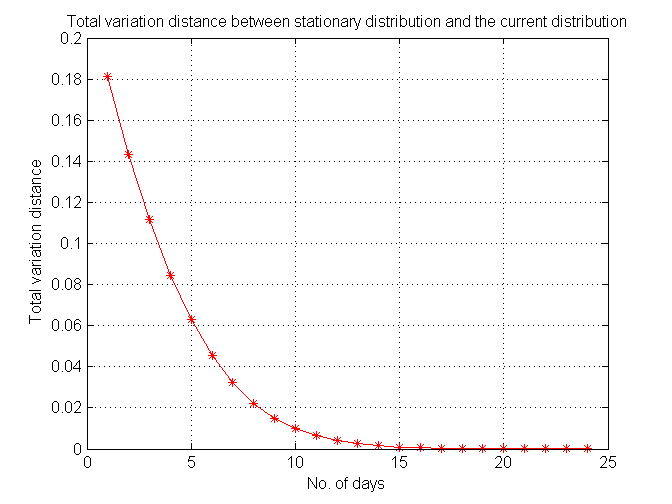
\includegraphics[width=.4\linewidth]{TVD1.png}
  %\caption{Total variation distance}
  %\label{fig:sub1}
\end{subfigure}
\begin{subfigure}
  \centering
  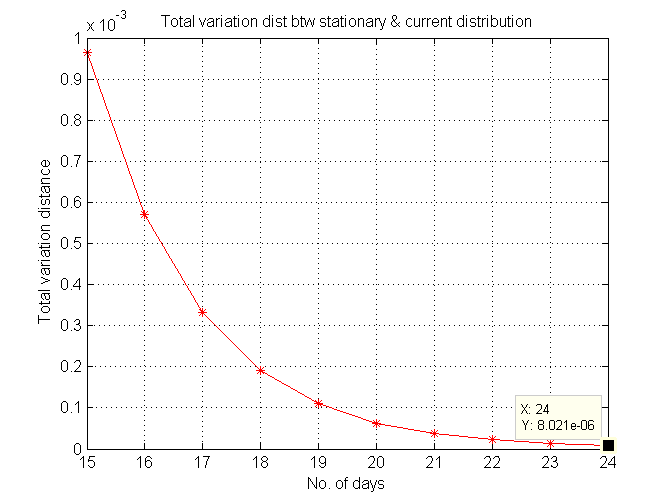
\includegraphics[width=.4\linewidth]{TVD2.png}
  %\caption{A subfigure}
  %\label{fig:sub2}
\end{subfigure}
\caption{Total variation distance}
\label{fig:test}
\end{figure}

From the above figure,obtained using MATLAB simulations, it can be observed that the total variation distance between the current distribution and the stationary distribution goes below 10$^{-5}$ for the first time on the 24$^{th}$ day.

\section{CONCLUSION}
The aim of this project was to model the effect of demonetization on consumption and predict the mean time by which economy stabilizes.We modeled cash-in-hand as a Discrete Time Markov Process. The changes in financial policies on withdrawal limits from November 2016 to February 2017 were observed. A different Transition Probability Matrix was constructed empirically for every change in policy using the data collected.As per the records in the website of Reserve Bank of India, by 20$^{th}$ February 2017, the withdrawal limits from banks and ATMs were restored.
\begin{itemize}
\item Under the assumption that TPM of the DTMC has become exactly the same as that before demonetization, the MATLAB simulations run by us indicated that by  16$^{th}$ March 2017, the economy  stabilized. Theoretical calculations suggests that the economy had stabilized by 13$^{th}$ March 2017.
\item We also considered another scenario in which TPM becomes a slighlty perturbed version of the one before demonetization.In this case, a lower bound on expected mixing time was found to 28 days,thereby indicating that economy could have stabilized only after 20$^{th}$ March 2017.
\end{itemize} 
\newpage
\section{APPENDIX}
From the data collected, the probability of consumption and withdrawal taking each value in state space were calculated empirically.Probability mass functions of withdrawal and consumption values are plotted below.
\\\\
\begin{figure}[H]
\centering
\begin{subfigure}
  \centering
  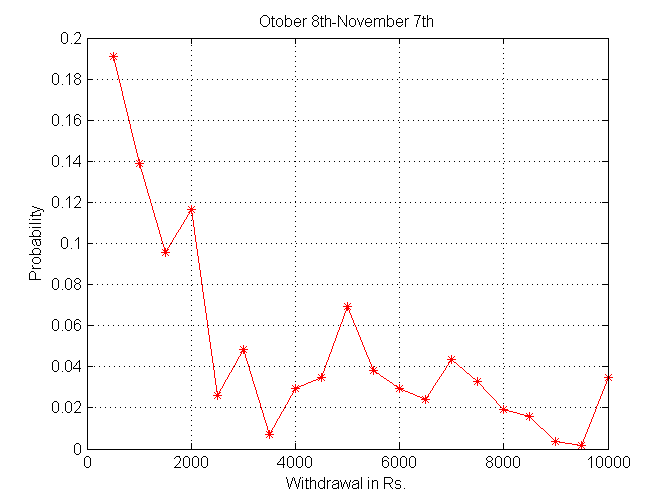
\includegraphics[width=.43\linewidth]{WOCT.png}
  %\caption{Total variation distance}
  %\label{fig:sub1}
\end{subfigure}
\begin{subfigure}
  \centering
  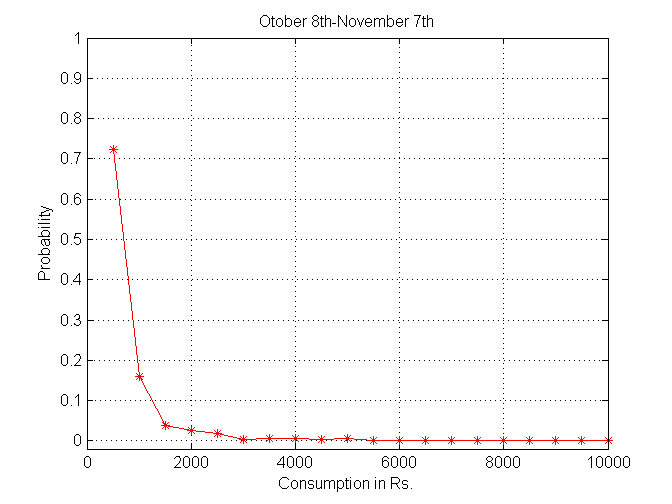
\includegraphics[width=.43\linewidth]{COCT.png}
  %\caption{A subfigure}
  %\label{fig:sub2}
\end{subfigure}
%\caption{Total variation distance}
\label{fig:test}
\end{figure}
\begin{figure}[H]
\centering
\begin{subfigure}
  \centering
  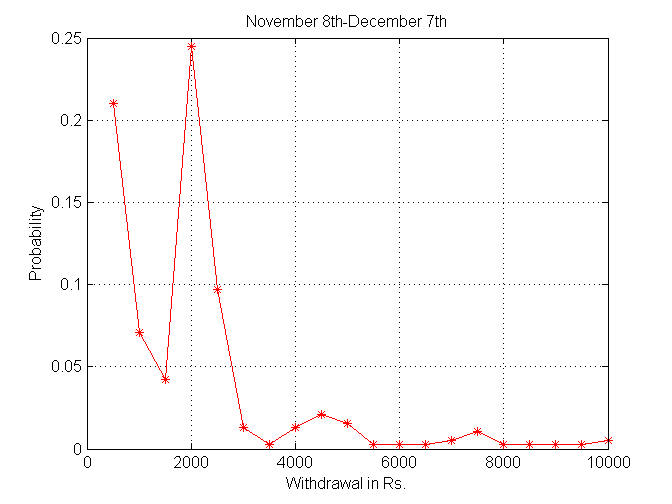
\includegraphics[width=.43\linewidth]{WNOV.png}
  %\caption{Total variation distance}
  %\label{fig:sub1}
\end{subfigure}
\begin{subfigure}
  \centering
  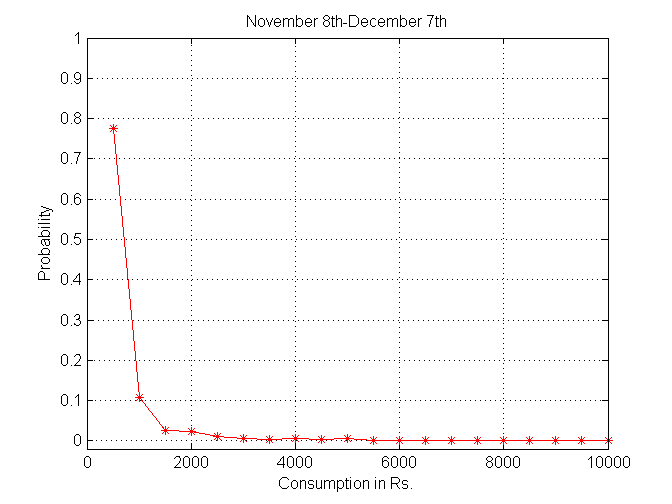
\includegraphics[width=.43\linewidth]{CNOV.png}
  %\caption{A subfigure}
  %\label{fig:sub2}
\end{subfigure}
%\caption{Total variation distance}
\label{fig:test}
\end{figure}
\begin{figure}[H]
\centering
\begin{subfigure}
  \centering
  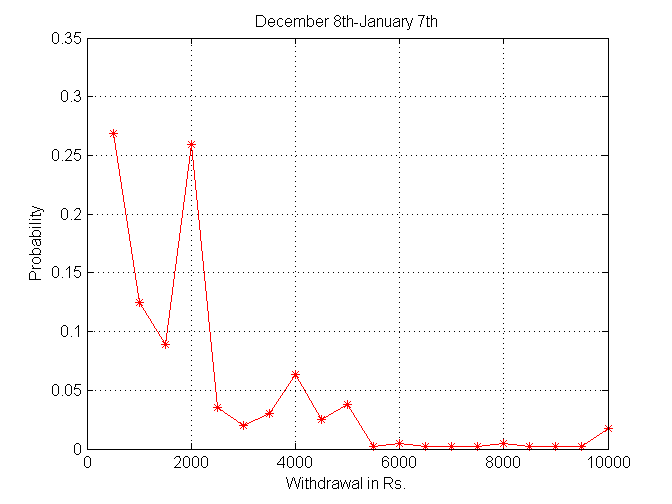
\includegraphics[width=.43\linewidth]{WDEC.png}
  %\caption{Total variation distance}
  %\label{fig:sub1}
\end{subfigure}
\begin{subfigure}
  \centering
  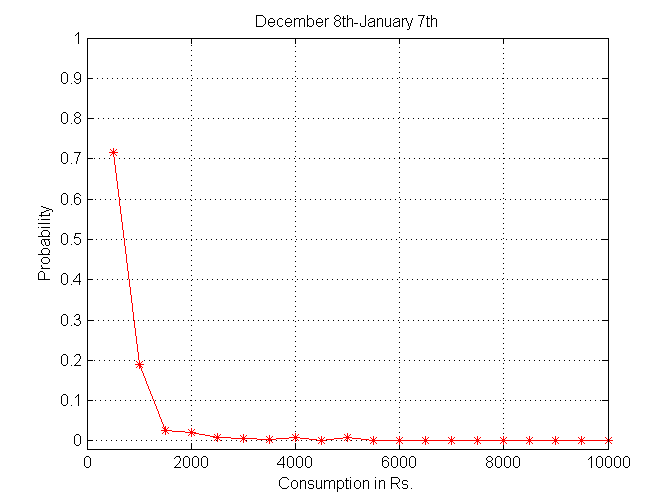
\includegraphics[width=.43\linewidth]{CDEC.png}
  %\caption{A subfigure}
  %\label{fig:sub2}
\end{subfigure}
%\caption{Total variation distance}
\label{fig:test}
\end{figure}
\begin{figure}[H]
\centering
\begin{subfigure}
  \centering
  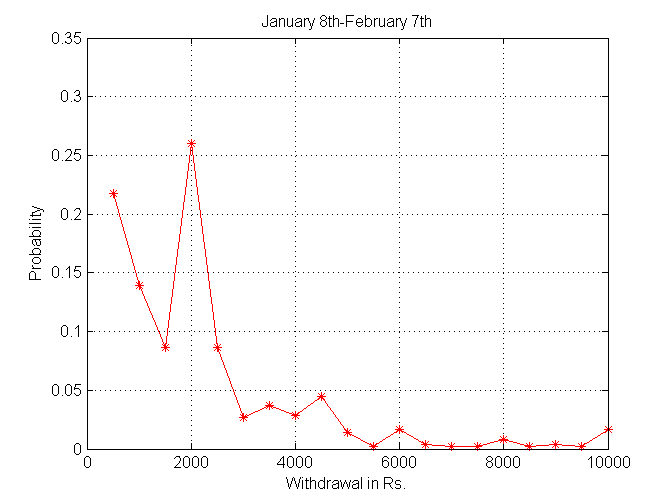
\includegraphics[width=.43\linewidth]{WJAN.png}
  %\caption{Total variation distance}
  %\label{fig:sub1}
\end{subfigure}
\begin{subfigure}
  \centering
  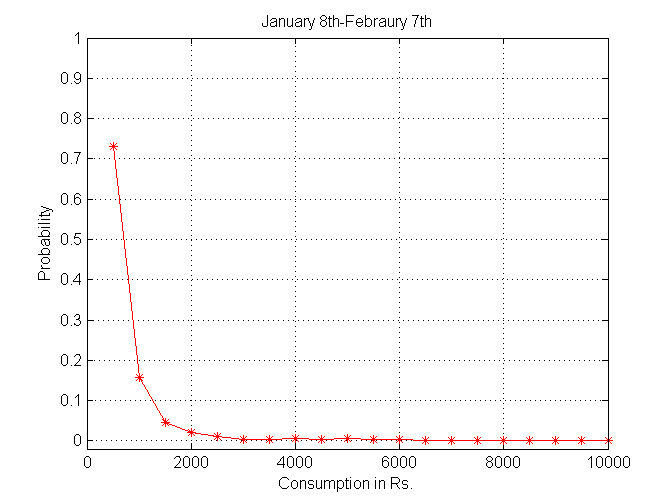
\includegraphics[width=.43\linewidth]{CJAN.png}
  %\caption{A subfigure}
  %\label{fig:sub2}
\end{subfigure}
%\caption{Total variation distance}
\label{fig:test}
\end{figure}
\newpage
\section{REFERENCE}
\begin{scriptsize}

\begin{small}
$[1]$ Jeffrey J. Hunter, "Coupling and Mixing times in Markov chains", Res.Lett.Inf. Math.Sci.(2007) 11, 1-22.\\
$[2]$ Hunter J.J., "Mixing times with applications to perturbed Markov chains", Linear Algebra Appl.,417, 108-123 (2006). \\
$[3]$ Hunter J.J., "Stationary distributions and mean first passage times of perturbed Markov chains, Linear Algebra Appl., 410 (2005) 217-243. \\
$[4]$ Robert E. Hall, "Stochastic implications of the life cycle-permanent income hypothesis:theory and evidence", Journal of Political Economy, 1978, Vol.86, No.6.
 \\
$[5]$ https://www.rbi.org.in/Scripts/NotificationUser.aspx\\
\end{small}
\end{scriptsize}




 







\end{document}
